%In this section we will detail the design of our tool, the algorithm and its parameters.
Our tool is implemented in Python. The language offers portability, access to rich libraries and fast development cycles. The disadvantages are speed and memory usage compared with compiled languages (e.g. C++) or newer scripting languages (e.g Julia).
Furthermore, Python's usage of a global interpreter lock makes shared memory parallelism not feasible. Distributed programming is possible using MPI.
\subsection{Algorithm}
%\subsubsection{Input and output}
The algorithm accepts a matrix X = n x k of input data, and a vector Y = 1 x k of expected data. It will evolve expressions that result, when evaluated on X, in an 1 x k vector Y' that approximates Y. N is the number of features, or parameters, the expression can use. We do not know in advance if all features are needed, which makes the problem statement even harder.
The goal of the algorithm is to find f' such that
\[Y = f(X)\]
\[Y' = f'(X)\]
\[dist(Y, Y') = e\]
results in e minimal. F is the process we wish to model or approximate with f'.\\
Not all distance functions are equally well suited for this purpose. A simple root mean squared error (RMSE) function has the issue of scale, the range of this function is [0, +$\infty$), which makes comparison problematic, especially if we want to combine it with other objective functions. A simple linear weighted sum requires that all terms use the same scale.
Normalization of RMSE is an option, however there is no single recommended approach to obtain this NRMSE. \\
In this work we use a distance function based on the Pearson Correlation Coefficient. Specifically, we define
\[
dist_p(Y, Y') = 1 - \vert r \vert
\]
with
\[
r = \frac{\sum_{i=0}^{n}{(y_i-E[Y])*(y'_i-E[Y'])}}{\sqrt{\sum_{j=0}^{n}{(y_j-E[Y])^2}*\sum_{k=0}^{n}{(y'_k-E[Y'])^2}}}
\]
R has a range of [-1, 1] where 1, -1 indicate linear and negative linear correlation respectively, and 0 indicates no correlation.
This function has a range [0,1] which facilitates comparison across domains and allows combining it with other objective functions.
The function reflects the aim of the algorithm. We not only want to assign a good (i.e. minimal) fitness value to a model that has a minimal distance, we also want to consider linearity between Y an Y'. The use of the Pearson correlation coefficient as a fitness measure is not new, a variant of this approach is used in \citep{pearson}.
\subsubsection{Genetic Programming Implementation}
We use Genetic Programming (GP) \cite{GP} to find solution to the problem statement. The algorithm controls a population of expressions, represented as trees, that are initialized, evolved using operators, and selected to simulate evolution.
The algorithm is subdivided in a set of phases, each phase initializes the population with a seed provided by an archive populated by previous phases or by the user. A phase is subdivided in runs, where each run selects a subset of the population, applies operators and if the application of the operator leads to fitness improvement replaces expressions. At the end of a phase the best expressions are stored in an archive to seed consecutive phases. At the end of a phases the best expressions are communicated to other processes executing the same algorithm with a differently seeded population. The next phase will then seed its population using the best of all aggregated expressions.
We use a vanilla GP implementation, with 'full' initialization method. Expressions trees are generated with a specified minimal depth. The depth of the expressions during evolution is limited by a second maximal parameter. GP differs from most optimization algorithms in this variable length representation. 
We use 2 operators in sequence, mutation and crossover. Mutation replaces a randomly selected subtree with a randomly generated tree. Mutation introduces new information, and leads to exploration of the search space. Crossover selects 2 trees based on fitness and swaps randomly selected subtrees. Crossover tends to lead to exploitation of the search space. Selection for crossover is random biased by fitness value. A stochastic process decides if crossover is applied pairwise (between fitness ordered expressions in the population) or at random.
The initialization of expression trees can lead to invalid expressions for the given domain. The probability of an invalid expression increases exponentially with the depth of the tree. A typical example of an invalid tree is division by zero. While some implementations opt for a guarded implementation, where division is altered in semantics to return a 'safe' value if the argument is zero, we feel that this alters the semantics of the results, and is somewhat opaque to the user. Our implementation will discard invalid expressions and replace them with a valid expression. Another approach is assigning a maximal fitness value to such an expression, but this can lead in corner cases to premature convergence when a few valid expressions dominate the population early on. We implement an efficient bottom up approach to construct valid trees where valid subtrees are merged. In contrast to a top down approach this detects invalid expressions early and avoids unnecessary evaluations of generated subtrees. Nevertheless, the initialization problem leads to a significant computational cost in the initialization stage of each phase and in the mutation operator.
\subsection{Distributed algorithm}
GP allows for both fine grained and coarse grained parallelism. Parallel execution of the fitness function can lead to a speedup in runtime, but will not alter the search process. Python's global interpreter lock and the cost of copying expressions for evaluation makes this approach unfeasible. A more interesting approach is coarse grained parallelism where we execute k instances of the algorithm in parallel and let them exchange their best expressions given a preset topology. The topology will determine both the convergence of the algorithm and the runtime.Exchanges of messages can introduce serialization and deadlock if the topology contains cycles. Our tool supports any user provided topology so must be able to deal with both issues effectively. 
After each phase a process looks up its targets given the topology. It then sends its best k expressions to the set of targets, either by copying all expressions to all targets or by spreading them over the target set. When the sending stage is complete, the process looks up its set of sources and waits until all source processes have sent their best expressions. To avoid deadlock a process sends its expressions asynchronously, not waiting until the receiving process has acknowledged receipt. The sent expressions are stored in a buffer for this purpose, together with an associated callable waiting object. After the sending stage the process synchronously collects messages from its sources, and executes the next phase of the algorithm. Before the next sending stage, the process will then check each callable to verify that all messages from the previous sending phase have been collected. Once this blocking call is complete, it can safely reuse the buffer and start the next sending phase. This also introduces a delay factor between processes. The phase runtime between processes will never be exactly identical, especially not given that the expressions have a variable length representation and differing evaluation cost. Without a delay factor processes would synchronize on each other, nullifying any runtime gains. With this delay factor a process is able to advance k phases ahead of a target process k steps distant in its topology. 
For hierarchical, non-cyclic topologies this can lead to a perfect scaling, where synchronization decreases as the number of processes increases.
\subsection{Approximated k-fold cross validation}
We divide the data over k processes with each process use a random sample of 4/5 of the total data. Each process operates on a further 4/5 split between training and validation data. The aggregate distributed process then approximates k-fold cross validation. Independent of the topology each randomly chosen pair of communicating processes will have the same probability of overlapping data. When this probability is too low, overfitting will be introduced and highly fit expressions from one process will have a high probability to be invalid for another process' training data. When the overlap is too great both processes will be searching the same subspace of the search space.
%
%\subsubsection{Diversity}\label{subsubdiversity}
%Diversity, the concept of maintaining semantically different specimens, is an important aspect in metaheuristics. Concepts such as niching and partitioning are often used to promote this behavior, amongst other reasons to prevent premature convergence or even to enable multimodality.
%Our tool uses a simple measure that approximates the more advanced techniques stated above. It should be clear that for any combination of input and output data, there are is huge set of expressions with identical fitness values. Such expressions can lead to premature convergence where a subset of the fittest expressions all have the same fitness value without introducing new information. Those expressions approximate the same local optimum. Our tool will aim to prevent retaining expressions that have identical fitness values.
%%Some metaheuristics \cite{DE} allow replacement of solutions with identical fitness values as it can help avoid local minima.
%There are disadvantages to this approach, if the fitness function has a zero gradient surface allowing replacement based on equal fitness value can help the optimizer to traverse such an area.
%
%\subsubsection{Predictive behavior}
%The algorithm evaluates expressions based on training data $X_t \subset X$. $X_t$ is an n x (rk) matrix sampled from the original input matrix X, with $r \in ] 0,1 [$.
%R is the sampling ratio, the ratio between training and validation data.
%After completion of the algorithm the population is ordered based on minimized fitness values calculated on the training data.
%In real world applications practitioners are also interested in the predictive qualities of the generated expression. In other words, how well do the expressions score on unknown data? In the final evaluation we score each expression on the full data to obtain this measure.
%While this gives us some information on how good an expression is on the full data set, we are also interested in how the convergence rate corresponds to the final fitness value on the full data.
%If we add 10 more generations, or increase the population by a factor 1.5, what do we gain or lose in predictive quality of the expressions?
%To define this we use a correlation measure between the fitness values using the training data and those of the full data.
%This measure quantifies the predictive value of the final results.
%Finally, we calculate a correlation trend between the training fitness values at the end of each phase, and the final fitness values calculated on the full data. This trend describes the convergence process of the algorithm over time, specifically directed at the predictive value of the solutions found. It is important to note that the entire final population is considered in these calculations, not only the best. While ideal, there is no guarantee that the expression that has the lowest fitness value on the training data will score best on the full data set. Using this correlation measure we can estimate how the convergence rate on the unknown data evolves over time. This measure then also serves as an indicator for overfitting.
%
%\subsubsection{Convergence limit}
%As a stopcondition our tool uses a preset number of iterations. The user specifies the number of generations (g) and phases (r), and the algorithm will at most execute g x r iterations. Convergence stalling is implemented by keeping track of the number of successful operations (mutation or crossover). If this value crosses a threshold value convergence has stalled and the algorithm is terminated. An alternative stopcondition is a minimum quality or fitness that should be achieved. This is very hard to estimate. The topology of the fitness function is highly problem dependent. The 'hardness' \citep{GPHardness} of the problem will determine the convergence rate. Given that the desired solution is not known, it is impossible for a practitioner to know in advance how much time the algorithm will need in order to obtain the desired quality of solution. It is even possible that the algorithm converges to a suboptimal value with a fitness value strictly greater than the desired value. For these reasons we opted for a simple but robust stopping condition.
%
%
%\subsection{Initialization}
%Initialization is done using the 'full' method \cite{GP}. The algorithm has a parameter initial depth, each new expression in the population is created using that depth. Unless the maximum depth is equal to the initial depth, the algorithm will quickly vary in depth, evolving an optimal depth.
%
%\subsubsection{Invalid expressions}\label{subsubinvalidexpressions}
%Generating a random expression is done by generating random subtrees and merging them. An important observation here is that randomly generated expressions can be invalid for their domain. The ubiquitous example here is division by zero. Several approaches to solve this problem exist. One can define 'safe' variants of the functions, in case of division by zero, returning a predefined value that will still result in a valid tree. The downside to this approach is that the division function's semantics are altered. A practitioner, given an expression, would have to know that some functions are no longer corresponding entirely to their mathematical equivalents, and what 'safe' values the implementation uses.
%The other option is assigning maximum fitness to an invalid expression. While simple, this approach needs a careful implementation. From a practical standpoint wrapping functions in exception handling code will quickly deteriorate performance.
%Our approach is a domain check for each function, and communicating by return value if the domain check failed thereby avoiding exceptions.
%
%\paragraph{Invalidity probability}
%We define the probability that a randomly generated tree of depth d, with n possible features, k possible base functions, and j data points as q. With more complex problems d will have to be increased. GP is also susceptible to bloat \cite{GPBloat}, increasing d even further. This issue will affect generation of subtrees in mutation. With more datapoints the probability of at least one leading to an invalid evaluation will increase. An increase in d will lead to an exponential increase in the number of nodes in the tree. A node can be either a basefunction or a leaf (feature or constant). For each additional node the probability q increases. We can conclude that q, while irrelevant for small problems and depths, becomes a major constraint for larger problem statements.
%
%\paragraph{Bottom up versus top down}
%There are two methods to generate a tree based expression : bottom up and top down. The top down approach is conceptually simpler, we select a random node and add randomly selected child nodes until the depth constraint in satisfied. The problem with this approach is that the expression can only be evaluated at completion, early detection of an invalid subtree is impossible.
%In contrast in a bottom up construction we generate small subtrees, evaluate them and if and only if valid merge them into a larger tree. This allows for early detection of invalid expressions. A downside of this approach is the repeated evaluation of the subtrees, which can be mitigated by caching the result of the subtree.
%
%\paragraph{Disallowing invalid expressions in initialization}
%We can generate random expressions and let the evolution stage of the algorithm filter them out based on their fitness value, or we can enforce the constraint that no invalid expressions are introduced. The last option is computationally more expensive at first sight, since the algorithm is capable by definition of eliminating unfit expressions from the population.
%This can lead to unwanted behavior in the algorithm itself. For high q values we can have a significant part of the population that is at any one time invalid. This can lead to premature convergence, similar to a scenario where the population is artificially small or dominated by a set of highly fit individuals. Another observation to make is that the algorithm will waste operations (mutation, crossover) on expressions that are improbable to contribute to a good solution.
%While more expensive computationally, we therefore prohibit the generation of invalid expressions in the initialization.
%
%%\subsection{Evaluation and cost}
%%Expression evaluation requires a tree traversal for each datapoint. In order to compare optimization algorithms across implementations practitioners can use as a measure the number of evaluations required to reach a certain fitness level. If this measure is used, one should take into account that not all evaluations are equal. With the trees varying in depth and density the evaluation cost varies significantly. Furthermore, evaluating "1 + 2" is computationally far less expensive than "log(3, 4)". A simple count of evaluation functions executed does not really reflect the true computation cost, especially when we consider the variable depth of the trees. Increasing the depth leads to an exponential increase in the number of nodes, and thus in the evaluation cost.
%%Our tool uses a complexity measure that takes into account the density of the tree and which functions are used. A tree comprised of complex functions will score higher in cost than a corresponding tree using simple multiplications and additions. Although this is an option, we do not use this measure in the objective function. We would like to observe the effect of this cost, but not have it directly influence the algorithm. There is no direct link between more complex functions and an optimal solution. In certain domains the argument can be made that more complex functions are more likely to lead to overfitting, or more likely to lead to invalid trees due to a smaller domain.
%
%\subsection{Evolution}
%In the evolution stage we apply two operators on (a selection of) the population. The operators are configured to constrain the depth of the modified trees, enforcing the maximum depth parameter.
%We trace the application of the operators during the execution using an effectiveness measure. Each time an operator application is able to lower the fitness of a tree, this measure increases. Using this measure we can gain insight when and how certain optimizations and modifications work inside the algorithm instead of simply observing the algorithm as a black box.
% \begin{figure}
%    \centering
%    \begin{subfigure}{0.5\textwidth}
%    \centering
%        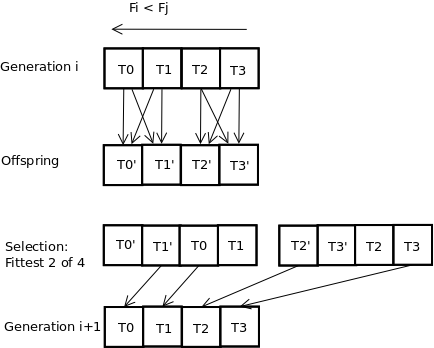
\includegraphics[width=0.8\linewidth]{figures/pairwisecrossover.png}
%        \caption{Pairwise crossover.}
%    \end{subfigure}
%    \begin{subfigure}{0.5\textwidth}
%    \centering
%        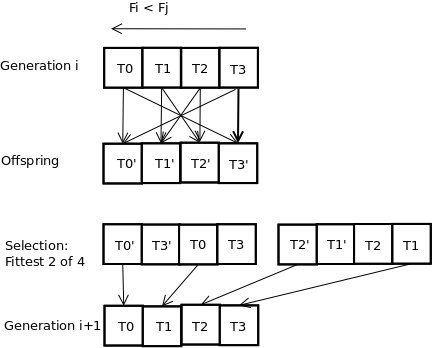
\includegraphics[width=0.8\linewidth]{figures/randomcrossover.png}
%        \caption{Random crossover.}
%    \end{subfigure}
%    \caption{Selection procedures applied by crossover.}
%    \label{fig:crossoverselection}
%\end{figure}
%
% \begin{figure}
%    \begin{subfigure}{0.5\textwidth}
%        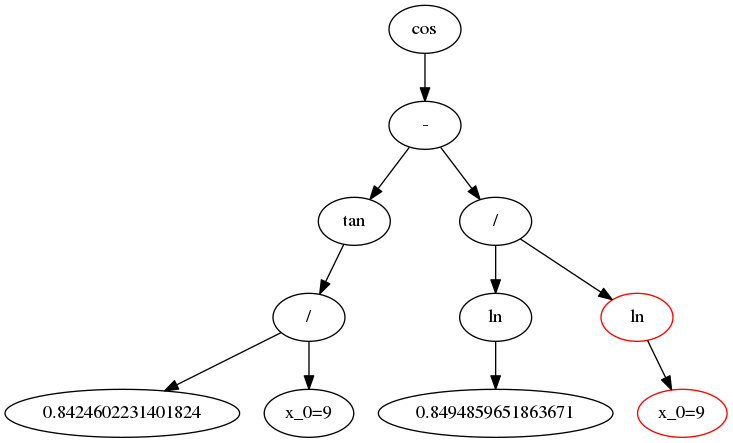
\includegraphics[width=0.8\linewidth]{figures/leftbefore.png}
%        \caption{A before crossover.}
%    \end{subfigure}
%    \begin{subfigure}{0.5\textwidth}
%        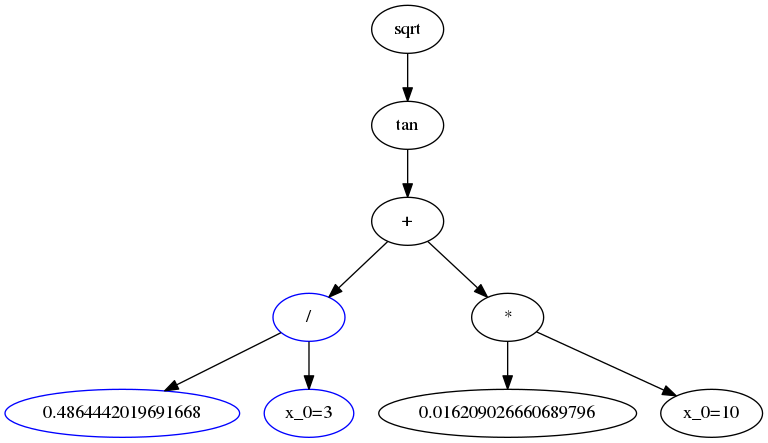
\includegraphics[width=0.8\linewidth]{figures/rightbefore.png}
%        \caption{B before crossover.}
%    \end{subfigure}
%        \begin{subfigure}{0.5\textwidth}
%        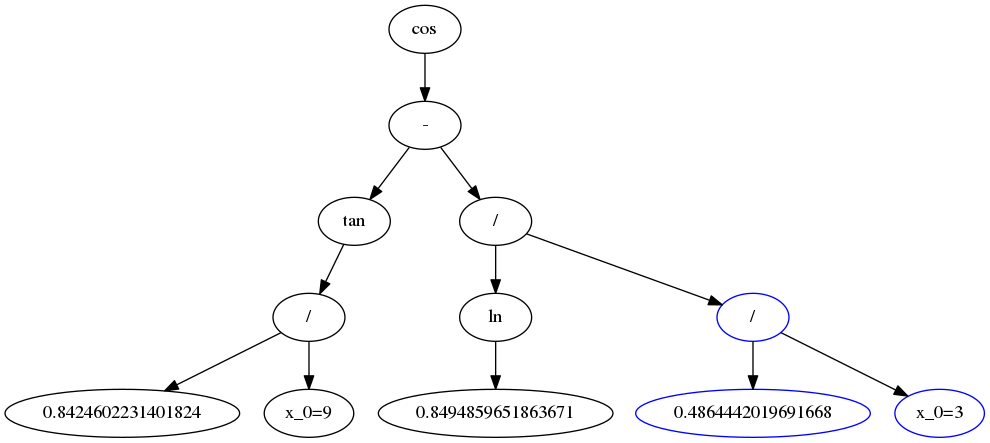
\includegraphics[width=0.8\linewidth]{figures/leftafter.png}
%        \caption{A after crossover.}
%    \end{subfigure}
%    \begin{subfigure}{0.5\textwidth}
%        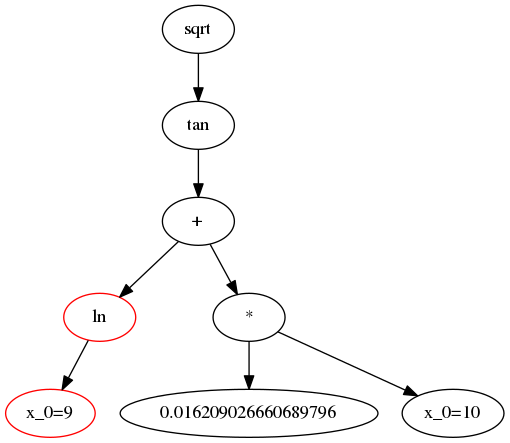
\includegraphics[width=0.8\linewidth]{figures/rightafter.png}
%        \caption{B after crossover.}
%    \end{subfigure}
%    \caption{Symmetric crossover with two random trees.}
%    \label{fig:crossover}
%\end{figure}
%
%\subsubsection{Mutation}
%Mutation works by replacing a randomly chosen subexpression with a newly generated expression. In our implementation this means selecting a node in the tree and replacing it with a new subtree. Our mutation operator can be configured to replace the subtree with one of equal depth or a randomly chosen depth. The insertion point can be made depth-sensitive. A shallow node, a node with a low depth, is the root of a subtree with significant depth. Replacing such a subtree is therefore more likely to have a significant effect on the fitness value. Replacing a deep node will have on average a smaller effect.
%The mutation operator is applied either selectively using a cooling schedule, or on the entire population.
%The cooling schedule uses the current fitness and the current generation of a tree to decide if the tree is likely to benefit from mutation. This is similar to the approach in simulated annealing \citep{SA}.
%Mutation introduces new information into the optimization process (a new subtree). This process can be constructive (lowering fitness) or destructive (increasing fitness). The idea behind the cooling schedule is that for fitter trees the mutation operation will not be able to improve fitness (decrease it), while for less fit trees it has a higher probability to do so.
%This probability is estimated using the current generation and fitness value (relative to the population), and using this information a biased random choice is made whether or not to apply mutation. In the experiments in section \ref{secexperiments} we will investigate if this assumption holds, and if it leads to gains in fitness and or effectiveness.
%The mutation operator has to generate new subtrees, and therefore the same issues seen in the initialization process which we discussed in section \ref{subsubinvalidexpressions} apply here as well. The mutation operator will generate subtrees until a valid one is found. If the depth sensitive operation proves to generate equal or better fitness values, this could significantly reduce the computation cost of the operator.
%
%\subsubsection{Crossover}
%Crossover operates on 2 trees in the population. It selects subtrees from both, and swaps them between each other. The resulting set of 4 trees is scored and the 2 fittest replace the original trees. As with mutation crossover can be configured to operate on a set depth, or select a random depth. It can also work symmetric, picking an equal depth insertion point in both trees.
%Crossover in our implementation can be applied in sequence to the entire population, with pairwise mating in order of fitness. Alternatively a random selection can be used. A variant of both, alternating between the two schedules based on a random choice is a third option. This is similar to the roulette wheel selection method, although without replacement.
%Crossover, unlike mutation, does not introduce new information in the sense that no new subtrees are generated.
%Crossover can be configured to work with a decreasing depth, operating only on deeper nodes at the later stages of the algorithm. The assumption for this mode of operation is similar to that made for mutation.
%In Figure \ref{fig:crossoverselection} we see both selection procedures visualized. An important difference with tournament selection is that there is no replacement used in our selection. Crossover will be applied to an expression exactly once.
%Crossover is based on the idea that 2 expressions can improve by combining parts of themselves. The operator is selecting these subexpressions randomly. Suppose we have 2 trees, A and B, with randomly selected subtrees a and b respectively. We do not know how much of the fitness of A is the result of its subtree a, and vice versa for B and b. In addition, we do not know or even are able to estimate if a will improve B's fitness value if we replace b with it. In Figure \ref{fig:crossover} we see this visualized for two random trees.
%If the expression represented by a tree is a set of separable functions we could use crossover and mutation only on those subexpressions. Unfortunately the search space is composed of both separable and non separable functions, and we do not know in advance if we gain from focussing only on separable solutions. Both crossover and mutation lack this information when dealing with subtrees and are forced to operate as random selectors.
%
%\subsection{Selection}
%After evolution a decision has to be made on which expressions to retain in the population. In our tool the population size is fixed, so a replacement is in order. We use an elitist approach. If an expression has a lower (better) fitness value after mutation, it is replaced.
%In crossover we combine two expressions r, and t, resulting in two offspring s, u.
%From these four expressions the two with minimal fitness survive to the next generation.
%
%\subsection{Archiving}
%The algorithm holds an archive that functions as memory for best solutions obtained from the best expressions at the end of a phase., from seeding, or from other processes.
%At the end of a phase we archive the j best expressions. J is a parameter ranging from 1 to the population size n. With j == n we risk premature convergence, with j == 1 the risks exists that we lose good expressions from phases which will have to be rediscovered.
%While there are numerous archiving strategies described in literature, we use a simple elitist approach. This means that there is no guarantee that the best j samples of phase i are retained, if they have fitness values lower than those present in the archive and the archive has no more empty slots, they will be ignored.
%This leads us to the size of the archive. While no exact optimal value for this exists, in order to function as memory between phases it should be at least equal to the amount of phases. The j parameter will influence this choice as well.
%
%%\subsection{Representation and data structures}\label{subsectree}
%%\subsubsection{Expression}
%%We use a tree representation for an arithmetic expression, where each internal node represent a base function (unary or binary), and each leaf either a feature or a constant.
%%
%%\paragraph{Tree representation}
%%We use a hybrid representation of a tree structure. The tree is a set of nodes, where each node holds a list of children nodes. This representation favors recursive traversal algorithms. In addition to this representation, the nodes of a tree are stored in a dictionary keyed on the position of a node. This allows for O(1) access needed by the mutation and crossover operators. The overhead of this extra representation is minimal, since the keys are integers and only a reference is stored. A list representation would be faster in (indexed) access, but would waste memory for sparse trees. With a mix of unary and binary operators the average nodecount of a tree with depth d is $\frac{2^{d+1}-1  + d}{2}$ = O($2^d$) resulting in savings on the order of $2^d$.
%%The algorithm has the choice which mode of access to use depending on the usage pattern. As an example, selecting a random node in the tree is O(1), selecting a node with a given depth is equally O(1). Splicing subtrees is equally an O(1) operation.
%%
%%\paragraph{Base functions}
%%The set of base functions is determined by the problem domain. For symbolic regression we use the following set:\\
%%+, -, \%, /, max, min, abs, tanh, sin, cos, tan, log, exp, power\\
%%A problem with this set is the varying domain of each, which may or may not correspond with the domain of the features. A possible extension is to use orthogonal base functions such as Chebyshev polynomials. In our solution the functions listed correspond with their mathematical equivalent, e.g. division by zero is undefined. Other constraints are based on floating point representation (e.g overflow).
%%
%%\paragraph{Constants}
%%Constants are fixed values in leaves in the tree. The representation also allows for multiplicative weights for each node, which can be used to further optimize an evolved expression. In contrast to the base functions with a limited set to choose from, constants have the entire floating point range at their disposal. The probability of selecting a 'right' value is extremely small, and domain information is lacking for these constants, it depends on the entire subtree holding the constant. We select a constant from a small range and allow the algorithm to recombine these constants later to larger values. This limiting of the search space can lead to the algorithm converging faster to a suboptimal solution.
%%The constants are reference objects in the tree, and so can be accessed and modified in place by an optimizer.
%%
%%\paragraph{Features}
%%Features are represented as an object holding a reference to a set of input values, and always occur as leaves. The choice for a random leaf is evenly distributed between constants and features.
%%
%%\subsubsection{Population}
%%The population of trees is kept in a sorted set, where the key is the fitness value and the value is a reference to the tree representing the expression.  Sorted datastructures are notably lacking from Python, we use the sortedcontainers \cite{sortedcontainers} module which provides sorted datastructures that are designed with performance in mind.
%%This representation allows for fast access in selecting a (sub)set of fittest trees. It also allows for an O(1) check to see if we already have an equivalent solution, a tree with a fitness score which we already have in the population. This allows our diversity approach mentioned in \ref{subsubdiversity}.
%%In Figure \ref{fig:uml} we see that the actual data structure used as population is interchangeable. If duplicate fitness values are allowed, and membership testing is no longer needed, a sorted list could be used instead.
%%
%%\subsection{Parameters}
%%In this section we briefly list the main parameters of the algorithm and their effects on convergence, runtime and complexity.
%%\subsubsection{Depth}
%%The depth of trees can vary between an initial and maximum value. If we know in advance that an optimal solution uses 13 features, the tree should have at least 13 leaves in order to use each feature at least once. This requires a depth of at least 4. In practice the depth will need to be greater due to the use of unary functions, and bloat. Bloat is a known issue in GP \cite{GPBloat}
%%where the algorithm, unless constrained by limits or an objective function that penalizes depth, will tend to evolve deep trees without gaining much in fitness. In the worst case entire subtrees can be evolved that do not contribute to the fitness value, similar to introns in genetics. These can still have a valid purpose, for example serving as genetic memory. Their disadvantage is clear: a computational overhead without clear effect on the fitness value.
%%A similar problem arises with the generation of constants. Suppose we would like to generate the constant 3.14, the probability of generating this by a single random call is extremely small. The algorithm will try to build an expression fitting 3.14, for example "1+(3*1) + 28/200". The problem with this is that this process is highly inefficient. It uses iterations that, if a more efficient approach exists, could be used to optimize the fitness value of the tree further. The constant expression wastes nodes that could be used to improve the tree. One approach is folding such expressions into a single constant, which mitigates some of the effects mentioned but does not prevent such subtrees from forming.
%%Without a solution for this issue, the user would have to take this into account and increase the depth parameter.
%%From \ref{subsubinvalidexpressions} we know that the initialization process and the mutation operator will become more costly exponential with the increase in depth.
%%The complexity of our tool is defined by the number of evaluations and the depth of the tree, with the depth having an exponential cost in time and memory.
%%
%%% complexity
%%\subsubsection{Population size}
%%The population size is directly related to convergence rate and the quality of the solution. A very small population will lead to premature convergence, the population is lacking in diversity (or information viewed from a different perspective).
%%A large population on the other leads to a large increase in runtime, unless the operators only work on a subset of the population. The optimal value is problem specific, but values in the range of [20,50] give a good balance for our implementation.
%%
%%\subsubsection{Phases and generations}
%%The execution of the algorithms comprises of g generations and r phases, resulting in a maximum of g x r iterations.
%%For both parameters a too small value will hinder convergence, while a high value can lead to overfitting. The optimal value is domain specific and dependent on the iterations required to approximate the expected data. This is by virtue of the problem statement unknown. There is a subtle difference between these parameters.
%%Each phase a reseed of the algorithm is done using the archive. This archive holds the best results from previous phases, external seeds and in a distributed setting the best best solutions from other processes.
%%The remainder of the population is initialized with a random tree. These trees introduce new information into the optimization process, and while expensive and with a low probability of improving fitness, nonetheless will help avoid premature convergence.
%%If the archive size is less than the population size, new trees will always be introduced. The rate at which the archive fills is dependent on the number of phases and a parameter which determines how many trees are archived. In a distributed setting this process is accelerated using the input of other processes. If the archive is full after i phases, and the archive size is equal to the population, further phases will no longer have the benefit of newly generated trees. This does not prevent convergence, but could reduce the convergence rate in some scenarios. Increasing g and r both can lead to overfitting, but in order to decide on r we also have to take into account the archiving strategy. In order to find a good starting value for g one can look at the population size.
%%Diffusion, where the information from each expression is shared with others, will require at least the same amount of generations as there are expressions, depending on the operators and the individual fitness of the expressions. Concentration, where we only look at maximizing the few existing fittest expressions, requires far less generations, but risks premature convergence.
%%\subsubsection{Samples}
%%The user can provide the algorithm with input data, or can specify a range from which to sample the input data. In addition, the ratio between training and testing data can be adjusted. Care should be taken in tuning this value. A low ratio will increase the probability that evolved solutions are invalid on the test data, while a high ratio will lead to overfitting.
%%
%%\subsubsection{Domain}
%%Domain specific knowledge can significantly reduce the time needed to converge to a solution. In our implementation we assume no domain knowledge. While this increases the complexity of obtaining a good solution, it also makes for a fairer evaluation of the algorithm and optimizations used.
%
%\subsection{Incremental support}\label{subsec:incremental}
%Our tool supports incremental operation. The user can provide seeds, expressions that are known or assumed to be good initial approximations. The algorithm writes out the best solutions obtained in an identical format. By combining this the user can create a Design Of Experiment (DOE) setup using the algorithm. As a use case, suppose the user wants to apply symbolic regression on the output of a computationally expensive simulation. The simulator has k features or parameters, each with a different domain and j datapoints. The user wants insights into the correlation of the parameters.
%A naive approach would be to generate output data for a full factorial experiment, and feed this into the CSRM tool. For both the simulator and the SR tool the cost of this approach would be prohibitive. It is likely that some features are even irrelevant, leading to unnecessary computation. Instead we can opt for a combined DOE approach. We start with a subset of features k' $<$ k and datapoints j' $<$ j. The simulation results Y' of this subset are then passed to the CSRM algorithm. It generates a set of solutions Q, optimized for this subset of the problem.
%The user then adds more parameters, k' $<$ k'' $<$ k and/or datapoints j' $<$ j'' $<$ j, runs the simulator again. The resulting output is given the CSRM tool, with Q as seed. This seed is used as memory of the previous run on the smaller input set. Unless there is no correlation between the incrementing datasets the CSRM tool can use the knowledge gained from the previous run to obtain faster convergence for this new dataset. In addition, by inspecting Q the user can already analyze a (partial) result regarding the initial parameter set.
%Suppose k = 5, and only 3 parameters are used in Q. Then the user can exclude the missing two parameters from the remainder of the experiment, as these are unlikely to contribute to the output. With a Latin Hypercube Design DOE approach the design would not have to be reconstructed in order to maintain a space filling design. We will detail this issue further in section \ref{secusecase}.
%By chaining the simulator and CSRM tool together in such a way, an efficient DOE approach can potentially save both simulation and regression time, or result in increased quality of solutions.
%The advantages are clear :
%\begin{itemize}
%\item The SR tool can start in parallel with the simulator, instead of having to wait until the simulator has completed all configurations.
%\item Intermediary results can be analyzed offering insights into the process that can be acted upon to alter the DOE.
%\item The SR tool can reuse previous results as seeds, restricting itself to a relatively small section of the search space instead of starting a blind search.
%\end{itemize}
%Possible disadvantages are :
%\begin{itemize}
%\item The SR tool is not guaranteed to return the optimal solution, it is possible the process is misguided by suboptimal solutions. This risk exist as well in the full approach.
%\item Interpretation of the results is needed in order to make the decision to prune features or datapoints.
%\end{itemize}
%We will investigate this approach in our use case in  section \ref{secusecase}.
%The diagram \ref{fig:incremental} illustrates a DOE hypercube design using our tool and a simulator. \\
%\begin{figure}
%\begin{tikzpicture}[node distance=1.5cm, every node/.style={font=\footnotesize}]
%\node (start) [startstop] {Start};
%\node (featureset) [process, below of=start] {Features};
%\node (datapoints) [process, below of=featureset] {Datapoints};
%\node (x) [process, right of= datapoints,xshift=4cm, yshift=1.5cm] {X};
%\node (simulator) [process, right of=x, xshift=4cm] {Simulator};
%\node (srtool) [process, below of=x] {CSRM};
%\node (y) [process, below of=simulator] {Y};
%\node (expressions) [process, below of=srtool] {Expressions};
%\node (analyze) [process, below of=datapoints] {Analyze};
%
%\draw [arrow] (featureset) -- +(+2,0) |-(x) node[near start,sloped,above]{};
%\draw [arrow] (start) --(featureset);
%\draw [arrow] (datapoints) -- +(+2,0) |-(x) node[near start,sloped,above]{};
%\draw [arrow] (x) --node[anchor=south]{input}(simulator);
%\draw [arrow] (x) --(srtool);
%\draw [arrow] (y) --(srtool);
%\draw [arrow] (simulator) --(y);
%%\draw [arrow] (simulator) -- +(0,-2) |-(srtool) node[near start,sloped,below]{Y};
%%\draw [arrow] (simulator) -- (srtool)node[anchor=east]{Y};
%\draw [arrow] (srtool) --node[anchor=east]{}(expressions);
%\draw [arrow] (expressions)-- +(-2,0) |- (srtool) node[near start,sloped,below, anchor=south] {seeds};
%\draw [arrow] (expressions)-- +(-2, 0) |- (analyze) node[near start,sloped,above, anchor=south] {};
%\draw [arrow] (expressions)-- +(-2, 0) |- (analyze) node[near start,sloped,above, anchor=south] {};
%\draw [arrow] (analyze)-- +(-2, 0) |- (featureset) node[near start,sloped,above, anchor=south] {};
%\draw [arrow] (analyze)-- +(-2, 0) |- (datapoints) node[near start,sloped,above, anchor=south] {reduces/expands};
%
%\end{tikzpicture}
%\caption{Incremental DOE using CSRM and a simulator.}
%\label{fig:incremental}
%\end{figure}
%
%\subsection{Statistics and visualization}
%Stochastic algorithms are notoriously hard to debug, analyze and reason about. By virtue of the problem statement we do not know whether the returned solution is what is expected. The size of the search space makes detecting all edge cases infeasible. In addition the algorithm functions as a black box, where output is presented to the user without a clear trace indicating how or why this output was obtained. For both developer and practitioner insight into the algorithms inner workings is vital.
%Our tool provides a wealth of runtime statistics ranging from fitness values per expression for each point in the execution, convergence behavior over time, depth and complexity of the expressions, cost of evaluations, effectiveness of operators, correlation between training and test fitness values and more. These statistics can be saved to disk for later analysis, or displayed in plots in a browser. Using this information the user can tune the parameters of the algorithm, for example reducing the number of phases when overfitting is detected. The developer can look at how effective modifications are to the operators, archiving strategy and so on.
%It is even possible to trace the entire run of the algorithm step by step by saving the expressions in tree form, displayed in an SVG image rendered by Graphviz \cite{graphviz}. In Figure \ref{fig:viz} a selection of the collected statistics on a testfunction is shown. The third of our set of testproblems was used with a depth $\in$ [4,10], 30 generations, populationsize 30, and 4 phases.
% \begin{figure}
%    \centering
%    \begin{subfigure}{0.5\textwidth}
%    \centering
%        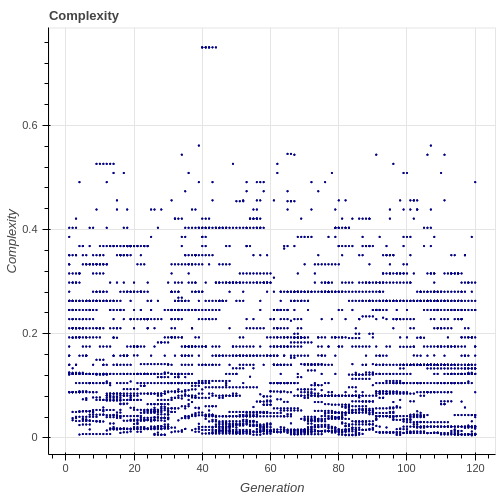
\includegraphics[width=0.8\linewidth]{figures/viz_complexity.png}
%        \caption{Scaled complexity over generations.}
%    \end{subfigure}%
%    \begin{subfigure}{0.5\textwidth}
%    \centering
%        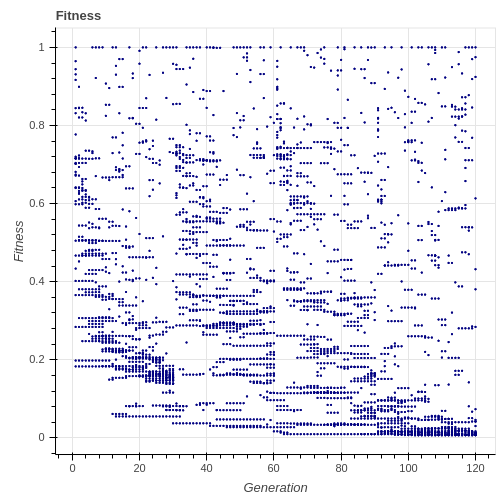
\includegraphics[width=0.8\linewidth]{figures/viz_fitness.png}
%        \caption{Fitness values over generations.}
%    \end{subfigure}
%        \begin{subfigure}{0.5\textwidth}
%    \centering
%        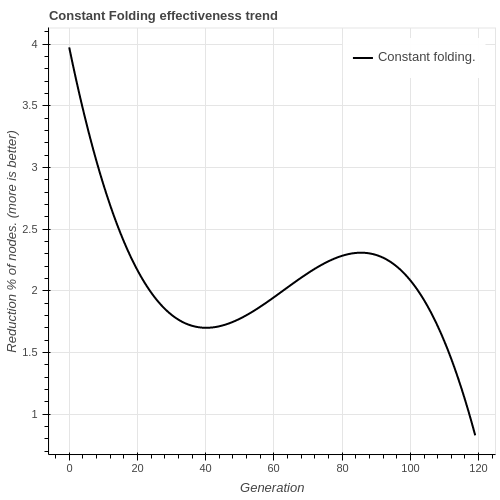
\includegraphics[width=0.8\linewidth]{figures/viz_constantfoldingtrend.png}
%        \caption{Constant folding savings.}
%    \end{subfigure}%
%    \begin{subfigure}{0.5\textwidth}
%    \centering
%        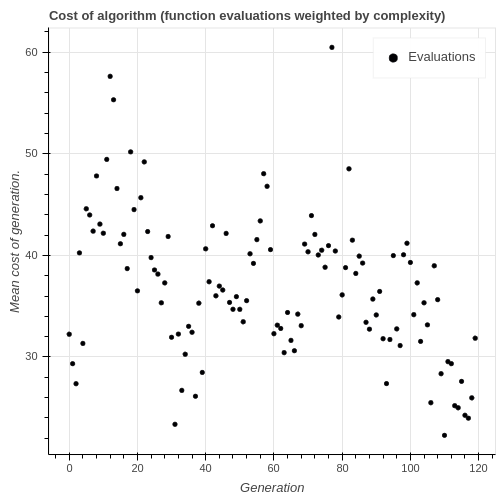
\includegraphics[width=0.8\linewidth]{figures/viz_meancost.png}
%        \caption{Mean evaluation cost.}
%    \end{subfigure}
%        \begin{subfigure}{0.5\textwidth}
%    \centering
%        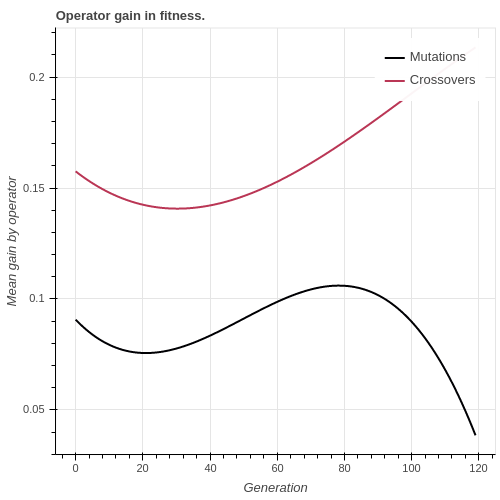
\includegraphics[width=0.8\linewidth]{figures/viz_operatorgaintrend.png}
%        \caption{Operator gain.}
%    \end{subfigure}%
%    \begin{subfigure}{0.5\textwidth}
%    \centering
%        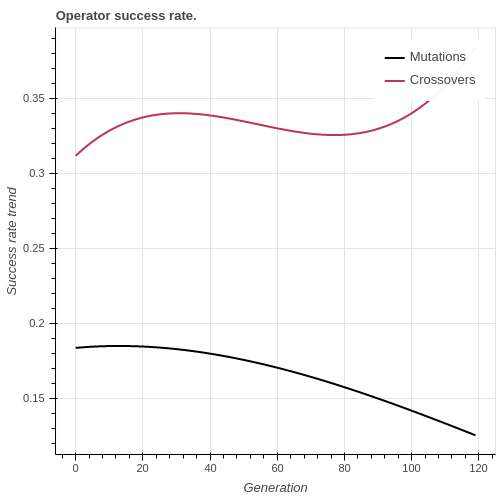
\includegraphics[width=0.8\linewidth]{figures/viz_operatorsuccessratetrend.png}
%        \caption{Operator success rate.}
%    \end{subfigure}
%    \caption{Selection of visualizations generated by CSRM.}
%    \label{fig:viz}
%\end{figure}
%
%%\subsection{Conclusion}
%%In this section we have covered in detail the design of the CSRM tool, highlighting the choices made. We have enumerated the features
%%% Full featured tool offers insight, variation, testing.
%%

%In this section we will cover the parallelization of symbolic regression, and detail the design choices we made in our approach.
%
%\subsection{Approaches}
%In this discussion we distinguish between fine grained parallelism and coarse grained parallelism. 
%
%\paragraph{Fine grained parallelism}
%In fine grained parallelism we parallelize a single step in the algorithm, where we execute a number of tasks in parallel that are independent of each other and where each task has a relatively short completion time. 
%The evaluation of the fitness function is a prime example of such a task. Evaluating fitness functions takes up the greatest part of the runtime in the algorithm.
%The fitness evaluation itself can be quite complex, but in comparison with the entire runtime of the algorithm the computational cost of a single calculation is small. In order to efficiently parallelize such a taskset we have to employ a mechanism that has minimum overhead. Shared memory parallelism using threads is ideal for this use case. Optimizations such as dynamically allocated threadpools will reduce the overhead even further, and thus increase the speedup. Overhead is split over the implementation overhead of starting, assigning and administering a thread, and the copying of the problem data and its solution. Shared memory implies a near zero cost in copying, only a reference is copied. A lock on the shared data is not needed since the instance the thread operates on is not used by any other part of the program while the fitness function is executed. This results in savings both in code complexity and synchronization overhead.
%
%\paragraph{Coarse grained parallelism}
%In coarse grained parallelism we run a series of tasks in parallel that have a long runtime or complex workload. In our setting an example of coarse grained parallelism is running the entire algorithm in parallel, with several instances tackling a distinct subset of the problem as separate processes. The significantly longer runtime of the task means that the overhead of parallelizing the problem can be significantly greater without impacting the speedup obtained. Typically we only start and stop such a task once, in contrast with fine grained tasks which are constantly started and then stopped again. We can use processes or threads for this form of parallelism. Threads have the benefit of being lighter in comparison to processes in terms of overhead. If we allow communication between the tasks threads can elide copying the data, at the cost of introducing locks. Processes typically have to copy data in order to communicate. We can compare both approaches with an interrupt based approach versus message passing. Whichever we choose, communication between tasks requires synchronization of some form. This introduces not only memory and time overhead, but also significantly complicates the implementation. Invariants that hold in sequential implementations are no longer guaranteed in parallel and a careful implementation is required. 
%
%\paragraph{Our approach}
%
%\subparagraph{Evaluating fine grained parallelism}
%Python has poor support for shared memory parallelism. While threading is available, it will not offer a speedup except for IO bound tasks due to the presence of global lock in the interpreter (GIL). It is possible to use compiled extensions in C to work around this issue, at a high cost in code complexity. A prototype implementation that parallelized the fitness function calculation proved that both threading and processes are unable to offer any speedup, often even running slower than sequential. A large part of this cost is due the overhead of copying Python objects, which are reference counted and thus require a graph traversal in order to create full copies. In order to evaluate a population of n expression trees of depth between 5 and 10 in parallel, we have to first copy the n expressions to each of the n processes, then evaluate the tree, and then copy the result back. The copying operation is orders of magnitude more expensive than the evaluation function, both scale exponentially in the depth of the tree. A prototype using threads elided the copy, but the GIL ensured that performance was still lower than the sequential approach.
%This ruled out fine grained parallelism in CSRM.
%
%\subparagraph{Evaluating coarse grained parallelism}
%We create k processes, and give each an instance of the algorithm to execute in parallel. Communication is done via message passing. We use the MPI framework, which offers Python bindings, to allow processes to communicate and synchronize. Copying is still costly, but now a speedup is possible. Threading did not work in this approach due to the GIL.
%CSRM uses a set of communicating processes in order to solve the distributed SR problem.
%
%\subsection{Distributed SR}
%We will now discuss the benefits of the distributed (coarse grained) application to our problem.
%
%\paragraph{Motivation}
%A parallel metaheuristic has the obvious advantage of speedup in comparison with a sequential implementation. By dividing the problem over k processes we can, in ideal circumstances, obtain a speedup linear in k. With speedup we then refer to the time, or number of evaluations, needed to reach a certain threshold of fitness. The advantages of parallelization do not stop with this speedup. We can view the parallel processes as a population based optimizer, where each instance communicates with the others using a predefined pattern. Instead of k standalone processes we now have a set of k cooperating  processes. Each process can now use the information of others to improve its own search. Using this approach a superlinear speedup is possible. There are, however, downsides. Communication implies overhead, not only in memory but also in synchronization. Without communication the only obstacle to obtain a linear speedup is dependent on the implementation. If we compare with the sequential process we need to clearly define measures to do so. If we run k processes, each with a population p, for g generations in r phases the entire process has executed k * p * g * r iterations. We cannot find an exact equivalent in the sequential algorithm. We could run the sequential algorithm k*r phases in order to simulate the same workload but the sequential and parallel algorithms will be different search processes. Increasing the phases or generations can easily lead to overfitting. Giving a sequential algorithm a population of k*p is not equivalent to the parallel algorithm. If we increase the population we need more generations and phases. If the number of generations is less than the population size not all expressions will have been able to use combine using crossover. Finally each of the k processes starts in a different part of the search space, on a different sample of the data. There is no direct translation between k parallel processes and a sequential process. 
%In this work we will focus on the effect a distributed approach has on the quality of the solution. We will measure the difference in quality of solution between the parallel implementations and the single sequential implementation and how it evolves over time. 
%
%\paragraph{Constraints}
%With communication we introduce synchronization constraints which can create a bottleneck for a subset of the processes, or in the worst case serialize the entire group. Our aim is to to exchange the most valuable information with the least amount of overhead. This balance is problem specific, the cost of copying depends on what exactly is being copied when and to whom it is sent. Even if we restrict ourselves to a 1-1 link between two processes, and only exchange the fittest expressions between the two processes, we do not know in advance how large the expression we copy will be, as the depth and sparseness of the tree representing the most fit expression will vary.
%While each process is given an equal sized subproblem, there are no guarantees that the actual workload of the different processes will be equal. We know that the evaluation of the fitness function has a variable computational load. The stochastic nature of the metaheuristics used in the SR implementation compound this issue. By virtue of the problem statement we do not know the optimal 
%solution to our problem, and with different starting points the convergence characteristics between the different processes are sure to differ. We will address each of these issues.
%
\subsection{Topologies}
A topology in this context is the set of communication links between the processes. The topology influences the convergence characteristics of the entire group. In a disconnected topology, there is no diffusion of information. If a process discovers a highly fit expression, that knowledge has to be rediscovered by the other processes in order to be used in the process. An edge case where this is an advantage is if we see the group of processes as a multiple restart version of the sequential algorithm. If the risk for premature convergence due to local optima is high, we can try to avoid those optima by executing the algorithm in k instances, without communication. Such an approach is sometimes referred to as partitioning, as we divide the search space in k distinct partitions.
%The implementation should offer the process an efficient way to lookup both processes from which it will receive information (sources) and processes it has to send to (targets). Source lookup is needed in order to solve the synchronization problem. Any topology that contains a cycle between processes can introduce a potential serialization effect at runtime.
%
\paragraph{Diffusion and concentration}
Our aim is for the processes to share information in order to accelerate the search process. With a topology we introduce two concepts : concentration and diffusion. Concentration refers to processes that share little or no information and focus on their own subset of the search space. Like exploitation concentration can lead to overfitting and premature convergence. It is warranted when the process is nearing the global optimum. Diffusion, in this work, is the spread of information over the topology. Diffusion accelerates the optimization process of the entire group. It is not without risk, however. If diffusion is instant, a single suboptimal solution can dominate other processes, leading to premature convergence. The distance between processes and connectivity will determine the effect diffusion has.
%The topology will determine the synchronization characteristics of the processes, as well as the balance between diffusion and concentration.
\paragraph{Grid}
The grid topology is 2 dimensional square of k processes with k a square of some natural number. Each process is connected with 4 other processes in north/south, east/west direction. The grid allows for delayed diffusion, to reach all processes an optimal expressions needs to traverse $\sqrt{k}$ links. This prevents premature convergence, with all processes still interconnected.
\paragraph{Tree}
A binary tree with with root as a source and leafs as sinks with unidirectional communication, the tree topology is an efficient example of a hierarchical topology. For k processes there are k-1 communication links, reducing the messaging and synchronization overhead significantly compared to the grid topology (4k). Diffusion can be hampered, each link is unidirectional so an optimal expression will not travel upwards to the root. On the other hand, with a spreading distribution policy where the optimal expressions are spread over the outgoing link, a partitioning effect will occur which can prevent premature convergence. There are no cycles, synchronization overhead is low.
\paragraph{Random}
In a random topology it is hard to predict how the convergence of the aggregated process will behave. It is possible that the topology contains cycles, but at the same time it can contain cliques. Diffusion is not guaranteed, and runtime performance will differ based on the actual instance. With grid and tree convergence and synchronization behavior is deterministic. The advantage of the random topology is that it can avoid certain patterns that occur in the other deterministic topologies. If the grid tends to lead to premature convergence for a given problem instance, it is possible that a random topology will avoid this.
%
%\paragraph{Synchronization}
%Synchronization between the processes will play an important role. While it does not directly influence convergence, it will constrain the runtime performance of the entire group. If we denote $S_i$ and $T_i$ as the set of processes that are sources and targets respectively for process i, we would like have $S_i$ minimal. The message processing code will have to wait for the slowest processes in $S_i$ before continuing. Without asynchronous communication process i would have to wait even longer, with the slowest process blocking the receipt of messages from the other processes. Synchronization implies that process i cannot send until its receiving stage has completed. If $S_i \cap T_i \neq \emptyset$ we have a cyclic dependency which can introduce deadlock in the implementation. By extension, if there is a cycle in the topology between any two processes deadlock is a real risk. Dealing with this in the communication code is non trivial. We will show in section \ref{subasync} how CSRM is able to deal efficiently with cycles in the topologies that it implements. Even with deadlock resolved, cycles will introduce a tendency for the the processes to serialize on the slowest process in the node. The time spent waiting in the communication stage is lost to the convergence process. We will show how this is mitigated in our implementation.
%
%\subsubsection{Grid}
%This topology arranges a set of k processes in a square two dimensional grid. Each process is connected with 4 neighbouring processes along the dimensional axes. Some variations include diagonal links, or create 3 or higher dimensional meshes. The general idea behind the grid remains invariant in those configurations. 
%A grid connects all processes, allowing for diffusion of the best solution to each individual process. The key observation here is that diffusion is gradual. While a process has an immediate neighbourhood, reaching all processes takes a variable amount of communication links. Diffusion of a dominating solution will take time, and if the solution is suboptimal this time allows the other processes to evolve their own optimal solutions thereby preventing premature convergence. This risk is only mitigated by gradual diffusion, not eliminated. Elimination is only possible in the extreme case by an absence of communication or in a more advanced configuration by the usage of cliques. 
%Nodes on the borders of the grid communicate with their counterparts at the mirrored side of the grid. This ensures that the communication process is symmetric. CSRM supports both square grids, where k is a square of a natural number, or incomplete squares. 
%If $\sqrt{k} \neq n $ for some $n \in \mathbb{N}$ we create a grid that would fit j processes with j given by 
%\[\forall j \in \mathbb{N} \min(j) > k \land \sqrt{j} = n \] 
%This grid is filled row by row with k processes. This configuration should be avoided, as the communication pattern will not always be symmetrical. It is implemented to allow a fair comparison with other topologies where the processcount is not a square and in the case where the number of processes is set by hardware limits or resource constraints.
%In Figure \ref{fig:topologies}\subref{subfig:grid} we see the communication pattern in a grid with 9 processes.
%
%\paragraph{Cost}
%The communication cost for k processes in a single iteration, with m messages sent per exchange, is in our configuration 4 mk.
%The synchronization constraints are high, all processes are interdependent (directly or at most $\sqrt{k}$ links removed).
%The lookup of targets is static, at configuration each parallel process is given a simple integer indexed mapping, the symmetry of this mapping simplifies the lookup code.
%
%\subsubsection{Wheel}
%A wheel or circle topology connects all processes with a single link shared between each source and target. Diffusion is slower than compared to the grid. For k processes it takes k-1 iterations for a message to reach all processes. Some variations introduce a 'hub', with spokes reaching out to the circle itself, completing the wheel analogy. CSRM implements this topology as a simple circle without hub or spokes. A spoked wheel topology, if the hub has bidirectional communication with all processes, has a maximum distance of 2 between all processes offering fast diffusion. Without a hub but with bidirectional links the maximum distance is $\frac{k}{2}$. A unidirectional variant is shown in Figure \ref{fig:topologies}\subref{subfig:wheel}.
%
%\paragraph{Cost}
%For k processes with m messages sent per exchange the communication cost is km. This is a static configuration with symmetric lookup. A circle is a cycle, this results in high synchronization constraints. The variant with hub and spokes introduces even higher synchronization constraints. At a doubling of message cost the doubly linked circle has an significantly higher synchronization cost than the singly linked variant. 
%
%\subsubsection{Random}
%In this topology a process selects a random target. We can configure it to do so statically, such that the target remains invariant at runtime, or select a new target after each phase. The number of targets is variable as well. CSRM implements all variants, allowing for both dynamic and static random topologies with a variable amount of targets per sending process. 
%The idea behind a random topology is that it avoids fixed communication patterns that are present in the structured topologies. If such a pattern leads to premature convergence, poor synchronization or fails to gain from the exchange of information between the processes there exists a possibility that a random approach can work. The downside is that we do not know what the maximum distance is between two processes, or even if they are connected. Cliques or cycles can form in the topology. Avoiding or detecting these requires more complex code than a simple random assignment of targets. By increasing the number of targets we decrease the probability for cliques while increasing the probability for cycles. Increasing targets will minimize the distance between two processes but increases synchronization and memory overhead.
%CSRM does not enforce constraints such as clique or cycle forming in its random topologies. In Figure \ref{fig:topologies}\subref{subfig:clique} we see how a clique of cycles created by a random static configuration. A configuration with 2 links per process is shown in Figure \ref{fig:topologies}\subref{subfig:randomstatic}.
%
%\paragraph{Cost}
%The cost for a singly linked random static topology of k processes with m messages per exchange is clearly km. Synchronization constraints are unknown, and would have to be resolved by the processes. Cyclic dependencies between the processes are likely.
%The lookup code for a static configuration is simple, symmetric and fast. For a dynamic configuration the lookup is simple, but only symmetric at single points in time. This observation is important because the virtual time of a process will diverge from that of the other processes. By allowing a dynamic configuration we introduce a new type of synchronization constraint. In CSRM processes have a copy of the global topology, but this is now no longer immutable. In order to resolve sources the process has to know the virtual time of the other processes. The topology remains deterministic, the seed used is identical between each process. Synchronization is highly complex in a random dynamic topology as cycles and cliques vary over time.
%
%\subsubsection{Tree}
%We introduce a binary tree topology. The links are unidirectional, with a single root and a given depth. The processcount should ideally be $k = 2^{d+1} -1$ for some $d > 0 \in \mathbb{N}$ to create a full binary tree. This is not a hard constraint, for values of not satisfying the constraint we construct a tree of depth $ d =\lfloor\log_2{k}\rfloor$ and fill the last level left to right until all processes are assigned a position. Communication is unidirectional, from the root to the leaves. This topology is free from cliques or cycles. The leaves act as sinks, while the root is a source. Lookup is fast, static and symmetric. Each process except the leaves has at most two targets, and one source (except the root). The tree topology offers a structured balance between diffusion and concentration. The distance between two processes ranges from 1 to $\log_2{k}$. In the case of leaves the distance is infinite. Note that depending on the communication strategy, each subtree can behave as a sink. The subtrees will not share information, instead they concentrate on distinct parts of the search space.
%A variant on this topology is a singly linked list, where the maximum distance is k. The problem with this topology is that its diffusion scales linearly with k. The full binary tree configuration is shown in Figure \ref{fig:topologies}\subref{subfig:tree}.
%An alternative to this configuration is an inverted tree. If we invert all edges we now have for a tree of depth d $2^d$ leaves as independent processes feeding their best expressions to $2^{d-1}$ nodes. Instead of each process receiving at most from 1 other process their best solutions, each non leaf process will now receive from at least two other processes. Diffusion in this topology is best described in terms of shared knowledge. As we go up the tree from the leaves each node progressively learns more of this shared knowledge. In this variant a node receives knowledge from both subtrees, instead of distributing it over its subtrees. The tree act as a lens with each root of a subtree as a focal point.
%
%\paragraph{Cost}
%For k processes and m messages per exchange (k-1)m messages are exchanged per iteration. Synchronization overhead is minimal, there are no cycles and a process is influenced at most by $\log_2{k}$ other processes and influences at most k-1. With the exception of a disconnected topology the tree topology allows for the fastest speedup compared with grid, random and circle. 
%The tree topology offers a structured alternative to the grid topology, with a staggered diffusion pattern. 
%The tree topology saves a factor 4 in messaging cost compared to the grid topology. While this factor is constant, its effects are significant. 
%For the same messaging cost a process in a grid topology can send trees of depth d, whereas in the tree topology it can send trees of depth d+2. This difference in depth allows for more expressive trees that can result in higher fitness value for the same communication cost. The disadvantage is that total diffusion is no longer possible.
%
%\subsubsection{Disconnected}
%The disconnected topology has zero diffusion and an infinite distance between processes. The only applications of this topology are in cases where the risk for premature convergence due to diffusion is high and can for some reason not be mitigated. Secondly it can serve as a comparison with the other topologies in order to measure the diffusion effect, memory and synchronization cost. 
%
%\paragraph{Cost}
%Cost is near zero, no messages are sent nor is any synchronization needed. In practice the collecting of all results will still have to be done by either an elected process or a process statically assigned as collector. This holds true for all topologies.

%\subsection{Asynchronous communication}\label{subasync}
%We have to tackle deadlock and synchronization delay in our parallel implementation. We will first describe the interaction between the processes and using this context demonstrate our solution.

%\paragraph{Control flow}
%The control flow of our parallel SR algorithm is shown in Figure \ref{fig:parallelflow}.
%A parallel process in our implementation executes a single phase of the algorithm, then collects at most m of its fittest expressions from the archive. 
%The set of target processes is resolved using the topology, then the m messages are sent to the targets. 
%After the sending stage the process looks up its sources using the topology, and waits for messages from those sources. 
%The received messages are decoded to expressions which are used by the algorithm for its next phase. The algorithm stores the expressions in its archive and then uses that archive to reseed the next phase. The archive is used for both external input and the best solutions from the previous phases. Since the archive has a fixed size, it will introduce an evolutionary pressure. A new expression will replace an existing if its fitness value is strictly lower. Allowing expressions with equal fitness values to replace each other can be useful in some cases where it allows the optimization process to traverse zero gradient areas in the topology of the fitness function. It can also lead to premature convergence where a large subset of the fittest population holds identical fitness values with low to no diversity. CSRM enforces a strict order in its population in order to prevent this last scenario. 
%
%\begin{figure}
%\begin{tikzpicture}[node distance=1.5cm, every node/.style={font=\footnotesize}]
%\node (start) [startstop] {Start};
%\node (phase) [decision, below of=start, yshift=-0.5cm] {Phase $<$ Phases};
%\node (execute) [process, below of=phase, yshift=-1cm] {0. Execute phase};
%\node (collect) [process, below of=execute] {1. Collect m best expressions};
%\node (lookup) [process, below of=collect] {2.0 Lookup targetset T};
%\node (spread) [process, below of=lookup] {2.1 Distribute m over T using policy};
%\node (check) [process, below of=spread] {2.2 Wait until all messages from previous phase have been received by target};
%\node (send) [process, below of=check] {2.3 Send m to t $\in$ T asynchronously};
%\node (lookups) [process, below of=send ] {3.0 Lookup sourceset S};
%\node (receive) [process, below of=lookups ] {3.1 Receive messages from s $\in$ S};
%\node (seed) [process, below of=receive ] {4. Reseed algorithm using received messages};
%
%\draw [arrow] (start) -- (phase);
%\draw [arrow] (phase) -- (execute);
%\draw [arrow] (execute) -- (collect);
%\draw [arrow] (collect) -- (lookup);
%\draw [arrow] (lookup) -- (spread);
%\draw [arrow] (spread) -- (check);
%\draw [arrow] (check) -- (send);
%\draw [arrow] (send) -- (lookups);
%\draw [arrow] (lookups) -- (receive);
%\draw [arrow] (receive) -- (seed);
%\draw [arrow] (seed)-- +(2,0) |- (phase) node[near start,sloped,above] {};
%\end{tikzpicture}
%\caption{Parallel control flow.}
%\label{fig:parallelflow}
%\end{figure}
%
%\paragraph{Waiting for messages}
%If a process does not wait for messages from other processes the convergence behavior of the entire group becomes non deterministic. In most platforms there are no hard guarantees about inter process scheduling. We can end up in extreme cases with a single process only sending and never consuming messages. This would break the intent of a structured topology. While this is an extreme example, even in average cases an extra level of non determinism is introduced without there being an explicit need for it. Not waiting for messages requires that messages are buffered by the parallel framework, and this can lead to internal buffers varying in size.  We will show another approach where the deterministic execution of the parallel metaheuristic is retained. This does not imply that the process itself is no longer stochastic, only that we are guaranteed that our designed communication pattern is strictly adhered to. Our algorithm can be provided with seeds making it deterministic. Each different seed is likely to lead to a different solution, or at least a different starting point. Without determinism it becomes very difficult to accurately compare configurations of the algorithm.
%
%\paragraph{Deadlock}
%From our previous discussion we know that deadlock is a risk if there are cycles in the topology. Since each process has full knowledge of the topology (except in a random dynamic topology) it is possible to implement an algorithm that resolves deadlock by ordering the sending and receiving of the messages. Suppose A waits for B, and B for A in the most simple example. A solution of A sending to B, B receiving from A, then B sending to A and A receiving from B would break the deadlock. This simple interleaving solution is not unique, but the priority is not important here. As long as the deadlock is broken the processes can continue. There are 2 serious issues with this approach. First, this approach serializes concurrent processes. This is detrimental to any speedup we were hoping to achieve. Second, the implementation becomes more complex. The order of calls is no longer statically defined, we need an algorithm that acts as a central coordinator between any group of processes in a cycle, computes a solution, and executes that solution in order. We cannot directly invoke operations on other processes, so the only solution is to execute the coordinating algorithm in parallel on all processes if they detect that they are a member of a cycle. Each process will then know when it can send and receive based on the computed order. While this solves deadlock, we still end up with a serialized execution and the communication code becomes far more complex than a simple sequential sending and receiving call.
%
%\subparagraph{Asynchronous solution}
%CSRM instead opts for an asynchronous sending of messages in order to resolve deadlock and mitigate serialization. Cycle detection is no longer needed. 
%A process executes a phase, then looks up its targets for messages. Instead of sending the messages with a blocking call to the framework, the sending process now allocates a buffer and sends each set of messages to its target with an asynchronous call. The messages are stored in the buffer until the receiver retrieves them. The sender stores a future object that can later be checked to verify if the receiving process has executed its receive call. 
%The order of sending is no longer relevant, the sending call returns immediately for each target. 
%Next the process calls receive for each of its sources. This is a blocking call, but this does not introduce a risk for deadlock. Invoking receive frees the buffer in the sender.
%In the worst case our process waits until the source has stopped its own sending call, but due to its asynchronous nature this process is quite fast. The order of sources is no longer a risk for deadlock. After receiving all messages the process continues its execution as before.
%Each process still has to clear the allocated buffers and callback objects from its send operation. The buffers cannot be deallocated as long as the receiving process has not acknowledged receipt of the contents. In order to check this we invoke the future objects, but care must be taken here. Calling the futures for each receiving process results in a blocking call. If we time this operation incorrectly we simply have deadlock all over again. The latest a process can wait is that point in time where the send buffers are needed again, which is in the next iteration. As soon as a process enters the sending phase, the first operation it executes is waiting on the future objects. After each returning call the corresponding buffer is cleared for reuse. 
%It should be clear that this approach does not simply delay deadlock but prevents it from occurring. The asynchronous approach allows the processes to interleave in any order that resolves the deadlock. Instead of an explicit algorithm, we simply let each cycle of processes resolve the deadlock in their own optimal sequence. Finally note that the receive call returns immediately once the framework has registered the corresponding send call, it is not directly waiting on the sending process.
%
%\paragraph{Synchronization delay}
%We know from our previous discussion that the execution time of a single phase will vary per process, and even between phases for a single process. The receiving of messages is a synchronization point between processes, but not a strict one as the sending process will only wait for receipt in the next phase. This means that a process will only be waiting on any other process after completion of a phase. If we introduce drift as the virtual time difference between processes then in order for processes to delay each other the drift would have to be greater than the execution time of a single phase. A strict serialization effect is avoided. What we introduce is a latency buffer equal to the runtime of the next phase. The time to execute a phase, while variable, will still be on average far greater than the time needed to communicate results. One of our aims in distributing SR is obtaining a speedup by, amongst other things, finding a balance between phase runtime and communication time.
%
%\subparagraph{Delay tolerance without cycles}
%In Figure \ref{fig:delaynoncyclic} we visualize how our approach allows a faster process to avoid waiting on a slower process. Solid vertical lines are blocking calls, the line represents the time spent waiting. The receive and check calls are blocking but return immediately. The send call is asynchronous and returns immediately. Asynchronous calls start the lifetime of a future object visualized with a vertical dotted line. The object's lifetime ends with a corresponding call from another process.
%The length of a phase is the delay tolerance that prevents strict serialization. We see three processes in a topology without cycles, where the phase time $t_p$ follows this pattern : $t_{pa} < t_{pb} < t_{pc}$. Process A can at most tolerate a delay of a single phase. If there is a strict ordering in average phase time between processes, then the processes will end up being serialized if the delay has exceeded a single phase. The average phase runtime will vary over time for a single process due to the ever evolving populations of differing depth and evaluation functions of varying complexity. The very fact that the runtime varies ensures that, with the exception of edge cases, the phase runtime average between processes will tend to the same values. Our approach allows the avoidance of serialization in the general case, given that the variation between the runtime will not be too extreme. The runtime of a single phase is dimensioned by the population and the number of generations. If we increase either one the runtime will increase, but the effect on the variation is far less predictable. In practice the runtime will depend on the average depth in the population and the average complexity of the population. With the depth limited the complexity is limited as well. The only remaining variable influencing runtime is then the scheduling algorithm of the operating system. With the exception of real time operating systems there is no upper limit here, but in practice the average runtime of a process on a system that is not overloaded will tend to a constant. This means that we can estimate a distribution of the phase runtime for a single sequential process, and use the mean and standard deviation of that distribution to find a value that prevents with a high probability serialization. 
%An important observation is that for a tree of depth d, the root process can be ahead of a leaf process at most d phases. This results in a staggered speedup effect. As the number of processes increases this speedup increases as well. The tree topology actually benefits from an increase in processes, unlike the other topologies.
%\begin{figure}
%    \centering
%    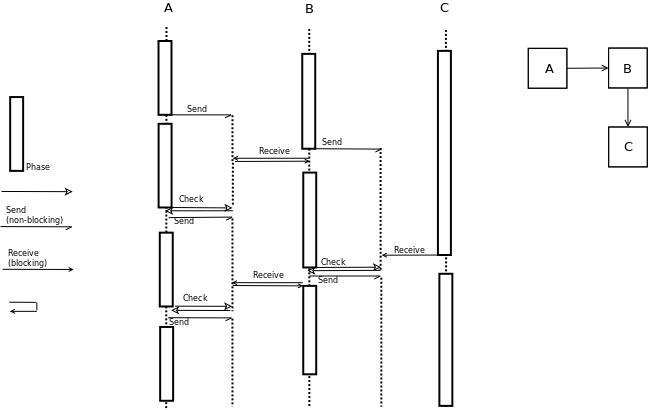
\includegraphics[width=\textwidth,height=\textheight,keepaspectratio]{figures/delay.png}
%    \caption{Synchronization delay tolerance in CSRM.}
%    \label{fig:delaynoncyclic}
%\end{figure}
%
%\subparagraph{Delay tolerance in the presence of cycles}
%When two processes have a cyclic dependency, where each waits on each other's communication directly or indirectly, the delay tolerance cannot avoid serialization. In Figure \ref{fig:delaycyclic} we see how processes A and B are serialized due to their interdependency. This cannot be avoided, process A needs the messages from B and vice versa in order to proceed. In the figure we see clearly the receive call waiting until a corresponding send call has been issued. While the send call returns immediately, the receive call has to block until send has been invoked. The same applies for the check call, until receive returns the check call blocks. In the figure the time spent waiting is visualized with a solid vertical line. 
%This figure demonstrates our deadlock resolution method. If the send call would block for either process, then both A and B would wait indefinitely. By making this operation return immediately the deadlock is resolved. This generalizes to larger cycles, for example in the wheel or grid topologies. Without this implementation only a tree topology or random topology with cycle detection could work.
%\begin{figure}
%    \centering
%    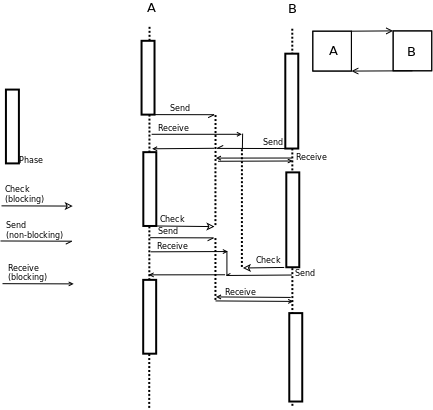
\includegraphics[width=\textwidth,height=\textheight,keepaspectratio]{figures/delaycycle.png}
%    \caption{Synchronization delay tolerance in CSRM in the presence of cycles.}
%    \label{fig:delaycyclic}
%\end{figure}
%
%\paragraph{Future improvements}
%If we allocate a buffer per communication phase, we can wait even longer before invoking future objects. This means we can execute a configurable amount of phases before we wait on the receipt of messages. The downside of this approach is that the memory constraints for each process now significantly increases from m to pm where p is the number of phases we opt to advance.
%The receive call is executed in sequence for the list of sources in the target process. In order to minimize delay even further we could execute this call asynchronously as well. Extra code would need to be introduced to handle the non deterministic behavior this introduces. The order in which the messages are received can influence the algorithm. When the archive is seeded with these external expressions we drop any expressions with identical fitness values. There is thus a risk that by varying the order we introduce non determinism in our results. This can be resolved in the receiving code by preallocating the buffer for all sources and after all asynchronous receive calls storing the messages in the same order of the sources list. 
%Asynchronous receiving is not implemented in CSRM.
%
%\subsection{Communication strategies}\label{subsec:commstrategies}
%If the process has j targets, and the algorithm is configured to distribute the m best solutions, we can use several approaches to send those to their targets. We can spread m over j, using a random, interleaving, slicing or any other type of sampling technique. An alternative is copying m j times so that each target receives the same m messages.
%CSRM has a Spreadpolicy interface that hides the implementation of this behavior for the processes. CSRM defaults to a slicing policy. If we have m messages to distribute over j targets, we will sequentially assign each of the j process $ \lfloor{m/j}\rfloor $ messages.
%This policy is efficient as it avoids copying but has a direct effect on the diffusion between the processes. First of all the value of m should be chosen with the topology in mind. With this policy a value of m = 2 for a grid pattern is problematic. A grid requires 4 outgoing messages. If we only send 2, the intended diffusion pattern is no longer valid. To avoid issues like this the spread policy will default to a copying strategy when m is insufficient for all links. In other words, m = 2 with 4 required messages will result in the m messages being copied to each outgoing link. 
%For a tree topology m should be 2 as well, else we create a symmetric series of cliques, which is unlikely to be intended. If we use a copy policy the value of m can be as low as 1. For random topologies m depends on the parameter determining the number of targets. In our circle topology m = 1 is sufficient for both policies.
%
%\begin{figure}
%    \centering
%    \begin{subfigure}{0.5\textwidth}\label{subfig:grid}
%	    \centering
%        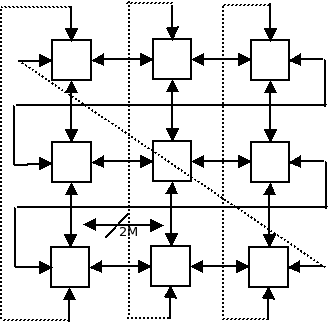
\includegraphics[width=0.6\linewidth]{figures/grid.png}
%        \caption{Grid topology with k = 9.}
%    \end{subfigure}
%    \begin{subfigure}{0.5\textwidth}\label{subfig:wheel}
%	    \centering
%        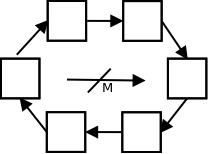
\includegraphics[width=0.6\linewidth]{figures/wheel.png}
%        \caption{Circle topology with k = 6.}
%    \end{subfigure}
%    \begin{subfigure}{0.5\textwidth}\label{subfig:tree}
%    \centering
%        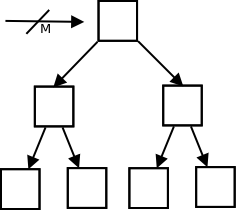
\includegraphics[width=0.6\linewidth]{figures/tree.png}
%        \caption{Tree topology with k = 7}
%    \end{subfigure}%
%    \begin{subfigure}{0.5\textwidth}\label{subfig:randomstatic}
%	    \centering
%		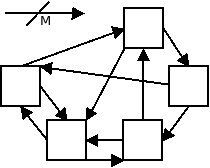
\includegraphics[width=0.6\linewidth]{figures/random.png}
%		\caption{Random topology with 2 outgoing links per process, k = 5.}
%    \end{subfigure}
%	\begin{subfigure}{0.5\textwidth}\label{subfig:clique}
%    		\centering
%        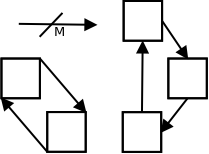
\includegraphics[width=0.6\linewidth]{figures/clique.png}
%        \caption{Random topology resulting in cliques of cycles, k = 5.}
%    \end{subfigure}%
%    \caption{Topologies in CSRM.}
%    \label{fig:topologies}
%\end{figure}
%
%\subsection{Exploiting parallelism for validation}
%
%\subsubsection{Predictive capability}
%In SR we try to find an expression that, based on some distance function, fits input data as close as possible to expected data. If we do not use test data to score the resulting expression, the risk of overfitting is very real. Not only is it possible that the expression fits the new data points from the test set poorly, the new datapoints may fall outside the domain of the generated expression. By scoring the expression on unknown data we measure its predictive capability $P_{sr}$. In sequential mode, CSRM evolves an expression on training data, then scores the expression on the full data. We record the correlation between the fitness on the training data and the fitness on the full data in order to measure, over generations and phases, the convergence process. We would like to have an answer to the question : How does $P_{sr}$ of the SR process evolve over time?\\
%This question is vital to a practitioner. If we have an indication that prediction is no longer increasing, or even decreasing we should halt the process. On the other hand if we see that a linear increase is still present we can opt for extending the runtime of the algorithm. Conventional validation, as described here, can be replaced with cross validation in order to obtain a more accurate measure for $P_{sr}$.
%
%\paragraph{Cross validation}
%Several approaches to cross validation exist. We distinguish between exhaustive and non-exhaustive methods. The first uses all possible combinations of training and test data to obtain the maximum amount of information of $P_{sr}$. Its disadvantage is a high computational cost, although this can still be linear in the length of the dataset if we omit only  a single datapoint per selection from the dataset. We will focus on k-fold cross validation (KCV), a non exhaustive validation technique. 
%In KCV we split the data over k samples, then use k-1 of those as the training data and one as the validation data. The process is repeated k times, to obtain full coverage. Even though this approach is non-exhaustive it would still require k iterations of the entire algorithm.
%
%\subsubsection{Parallelization}
%
%\paragraph{Approximating k fold cross validation}\label{KCV}
%With the distributed implementation of SR we can avoid the factor k increase required for KCV. CSRM can, as we have shown, run n instances of the algorithm in parallel. Those instances can cooperate by exchanging their current best solutions, possibly accelerating the convergence of the entire process. Instead of translating our sequential approach to the distributed approach and giving each process the same training data, we can approximate KCV without the linear increase in runtime. For a dataset of length d, KCV will split it into k equal sized sections of size s = $\frac{d}{k}$. Each training set has $s*(k-2)$ overlapping datapoints. The value of k determines the effect of the outcome to a large extent, allthough the sampling strategy is not unimportant either. We would like to keep the overlap above a certain treshold, insensitive to k. If the overlap is too small the probability of highly fit expressions proving to be invalid on the validation data becomes too large. 
%
\begin{figure}
    \centering
    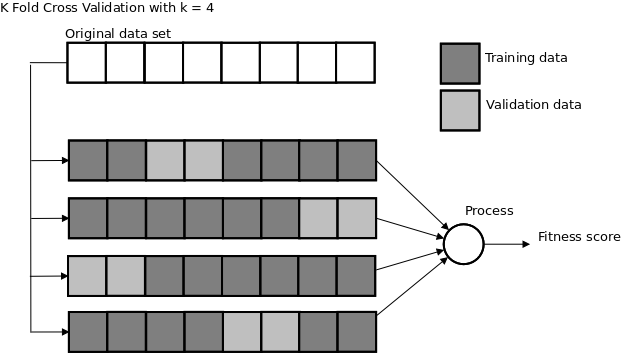
\includegraphics[width=\textwidth,height=\textheight,keepaspectratio]{figures/kfold.png}
    \caption{Visualization of k fold cross validation with k = 4.}
    \label{fig:kfold}
\end{figure}
%
%\paragraph{Approach}
%With k processes running in parallel, and d datapoints, we give each process a random sample of size r*d with $r \in ] 0,1 [$. In practice we use r = $\frac{4}{5}$. This is the same approach we use in our sequential implementation. The difference now is that each process is given a different trainingset of size r*d, with a stochastically determined overlap threshold. Each process uses its own distinct trainingset to evolve expressions from and at the end of its execution scores its population on the full data set. Each process uses a different seed for its random number generators, so we have k processes working on a different area of the search space, but there is enough shared information to make the results of each individual process relevant to each other. Our approach is visualized in Figure \ref{fig:csrmkfold} with $r = \frac{3}{4}$ and k = 4.
%The probability that any two trainingsets share a single datapoint is $r^2$. This probability is invariant to k, the number of processes. So for any two communicating processes, regardless of the topology or validation process, the ratio of shared data points is constant. When two processes exchange their best expression, the new expression is scored using the receiving process' training data set. The invalid expression problem is not only present at the end of the algorithm, it is also a vital factor during the communication between the processes. If process A evolves an expression that has a high probability of being invalid on process B's trainingset, the possible gain we have in sharing that expression evaporates. By establishing a constant threshold we can mitigate this risk and still gain from the validation process.
%The choice of concurrent processes is constrained in practice, typically it is determined by the available hardware or the topology. Our validation approach is insensitive to this value. 
%
%\begin{figure}
%    \centering
%    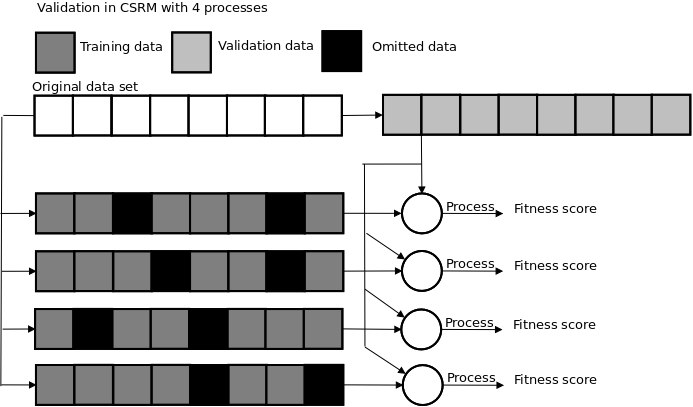
\includegraphics[width=\textwidth,height=\textheight,keepaspectratio]{figures/validationcsrm.png}
%    \caption{Approximation of k fold cross validation with parallel processes, k = 4,  r = $\frac{3}{4}$.}
%    \label{fig:csrmkfold}
%\end{figure}

\begin{figure}
	\begin{subfigure}{0.5\textwidth}\label{fig:csrmkfold}
    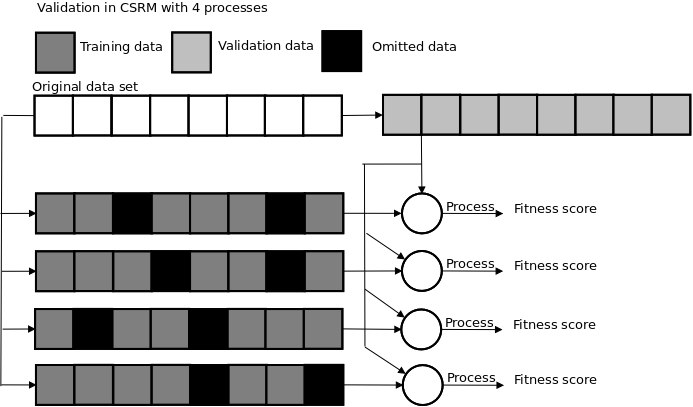
\includegraphics[width=\textwidth,height=\textheight,keepaspectratio]{figures/validationcsrm.png}
    \caption{Approximation of k fold cross validation with parallel processes, k = 4,  r = $\frac{3}{4}$.}
    \end{subfigure}
	\begin{subfigure}{0.5\textwidth}    \label{fig:kfold}

    \centering
    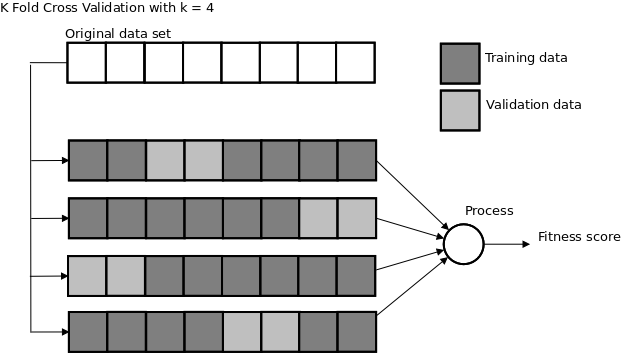
\includegraphics[width=\textwidth,height=\textheight,keepaspectratio]{figures/kfold.png}
    \caption{Visualization of k fold cross validation with k = 4.}
    \label{fig:kfold}
    \end{subfigure}%
    \caption{Topologies in CSRM.}
    \label{fig:ckfold}
 \end{figure}
%
%\subsection{Conclusion}
%We have covered our distributed design and highlighted the issues that drove our choices. CSRM offers the practitioner several topologies each with its strengths and weaknesses. 
%With a wealth of topologies and configurations we also increase the dimensions of the parameter optimization problem. In the experiments we will evaluate some, but not all parameter choices. 
%Our implementation can easily be extended with more topologies or policies without risking deadlock or serialization.
%Our validation approach in parallel CSRM allows an approximation of KCV without increasing the runtime cost by a factor k. The validation is insensitive to the number of processes and finds a balance between generating predictive expressions while minimizing the occurrence of invalid expressions.